\documentclass[border=10pt]{standalone}

\usepackage{tikz}
\usepackage{tikzsymbols}
\usetikzlibrary{calc,patterns,shapes.geometric}

\def\centerarc[#1](#2)(#3:#4:#5){\draw[#1] ($(#2)+({#5*cos(#3)},{#5*sin(#3)})$) arc (#3:#4:#5);}

\begin{document}
	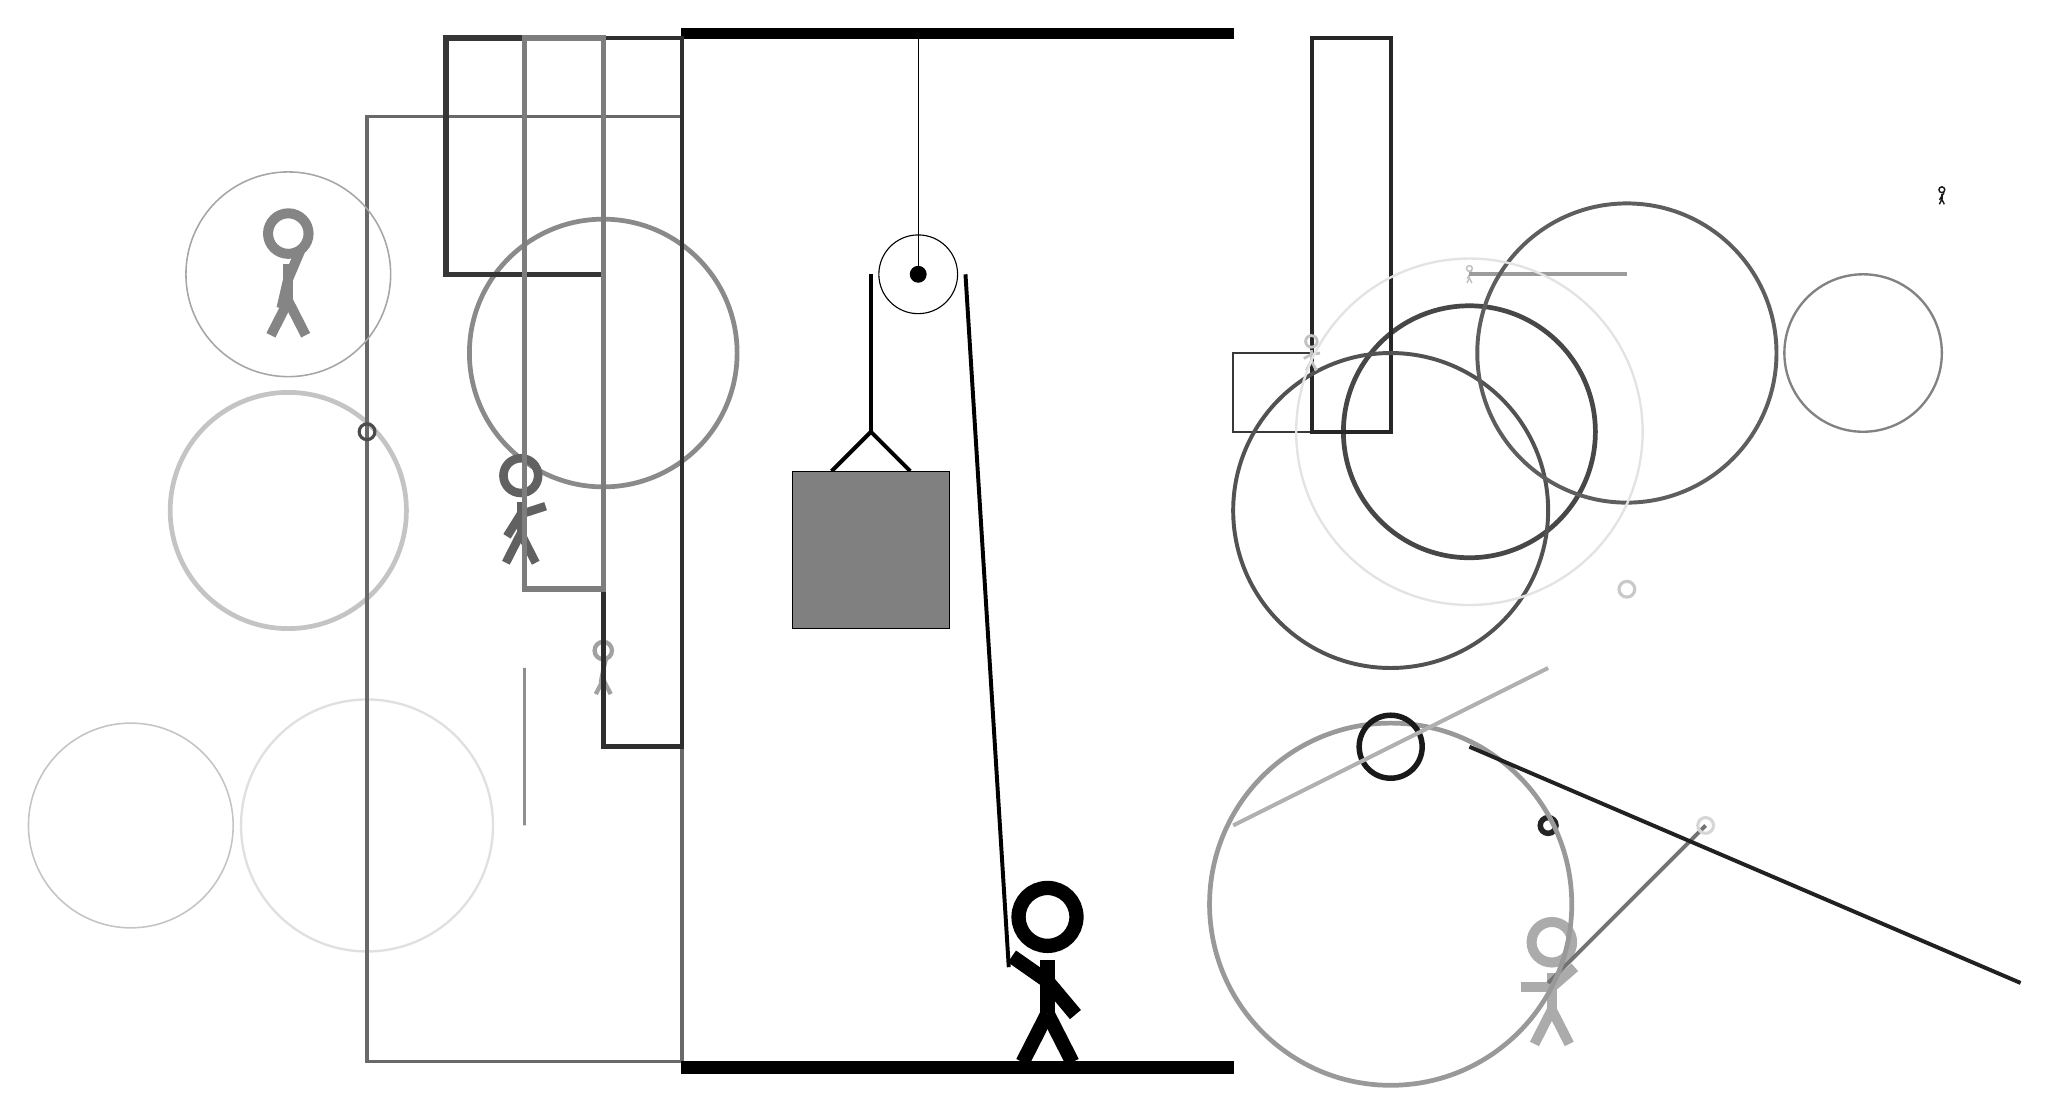
\begin{tikzpicture}
		%%%%% START %%%%%
		
		\draw[fill=black] (-2, 10) rectangle (5, 10.125);
		
		\draw (1, 7) circle (0.5);
		\draw[fill=black] (1, 7) circle (0.1);
		\draw (1, 10) -- (1, 7);
		
		\draw [line width=0.6mm, color=black!46](-3, 6) circle (1.7);
		
		\node[line width=0.5mm, color=black!48] at (-7, 7) {\Strichmaxerl[7][77][67]};
		\draw [line width=0.7mm, color=black!86](9, 0) circle (0.1);
		\draw[line width=0.3mm, color=black!78] (5, 5) rectangle (6, 6);
		\draw [line width=0.6mm, color=black!72](8, 5) circle (1.6);
		\draw [line width=0.4mm, color=black!21](10, 3) circle (0.1);
		\node[line width=0.2mm, color=black!33] at (9, -2) {\Strichmaxerl[7][0][41]};
		\draw[line width=0.5mm, color=black!85] (7, 5) rectangle (6, 10);
		\draw [line width=0.6mm, color=black!23](-7, 4) circle (1.5);
		\draw [line width=0.3mm, color=black!12](-6, 0) circle (1.6);
		\draw [line width=0.5mm, color=black!68](7, 4) circle (2.0);
		\draw[line width=0.5mm, color=black!55](9, -2) -- (11, 0);
		\node[line width=0.7mm, color=black!25] at (8, 7) {\Strichmaxerl[1][59][53]};
		
		\draw [line width=0.6mm, color=black!40](7, -1) circle (2.3);
		\draw[line width=0.5mm, color=black!39](8, 7) -- (10, 7);
		\node[line width=0.6mm, color=black!91] at (14, 8) {\Strichmaxerl[1][58][59]};
		\draw [line width=0.3mm, color=black!49](13, 6) circle (1.0);
		\draw [line width=0.2mm, color=black!23](-9, 0) circle (1.3);
		\node[line width=0.3mm, color=black!24] at (6, 6) {\Strichmaxerl[2][29][8]};
		\draw[line width=0.4mm, color=black!59] (-2, 9) rectangle (-6, -3);
		\draw [line width=0.5mm, color=black!63](10, 6) circle (1.9);
		\draw [line width=0.7mm, color=black!90](7, 1) circle (0.4);
		\draw[line width=0.5mm, color=black!31](9, 2) -- (5, 0);
		\draw[line width=0.7mm, color=black!79] (-3, 10) rectangle (-5, 7);
		\draw [line width=0.4mm, color=black!16](11, 0) circle (0.1);
		\draw [line width=0.2mm, color=black!35](-7, 7) circle (1.3);
		
		\node[line width=0.2mm, color=black!37] at (-3, 2) {\Strichmaxerl[3][79][76]};
		\draw[line width=0.3mm, color=black!44] (-4, 0) rectangle (-4, 2);
		
		\draw [line width=0.4mm, color=black!70](-6, 5) circle (0.1);
		\draw[line width=0.5mm, color=black!87](8, 1) -- (15, -2);
		\node[line width=0.7mm, color=black!62] at (-4, 4) {\Strichmaxerl[6][58][18]};
		
		\draw[line width=0.6mm, color=black!82] (-3, 1) rectangle (-2, 10);
		\draw [line width=0.3mm, color=black!11](8, 5) circle (2.2);
		\draw[line width=0.7mm, color=black!51] (-3, 3) rectangle (-4, 10);
		
		\draw[line width=0.5mm] (-0.1, 4.5) -- (0.4, 5.0) -- (0.9, 4.5);
		\draw[fill=black!50] (-0.6, 4.5) rectangle (1.4, 2.5);
		
		\draw[line width=0.5mm] (0.4, 7) -- (0.4, 5.0);
		\centerarc[line width=0.5mm](1, 7)(0:180:0.6);
		\draw[line width=0.5mm](1.6, 7) -- (2.15, -1.8);
		
		\node at (2.6, -1.9) {\Strichmaxerl[10][-35][-50]};
		
		\draw[fill=black] (-2, -3) rectangle (5, -3.15);
		
		%%%%% END %%%%%
	\end{tikzpicture}
\end{document}